% -*- TeX -*-
\documentclass[aspectratio=169]{beamer}

\usepackage{bm}
\usepackage{mathtools} % equations
\usepackage{booktabs}

\title{PyLith v3.0 Tutorial}
\subtitle{Introduction to PyLith v3.0}
\author{Brad Aagaard \\ Charles Williams \\ Matthew Knepley}
\institute{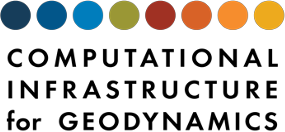
\includegraphics[scale=1.5]{../../logos/cig_logo_dots}%
  \hspace{4em}%
\raisebox{1em}{\includegraphics[scale=1.0]{../../logos/cig_short_pylith}}}
\date{June 20, 2022}


% ---------------------------------------------------- CUSTOMIZATION
\usetheme{CIG}
% Style information for PyLith presentations.

% Colors
\definecolor{ltorange}{rgb}{1.0, 0.74, 0.41} % 255/188/105
\definecolor{orange}{rgb}{0.96, 0.50, 0.0} % 246/127/0

\definecolor{ltred}{rgb}{1.0, 0.25, 0.25} % 255/64/64
\definecolor{red}{rgb}{0.79, 0.00, 0.01} % 201/0/3

\definecolor{ltpurple}{rgb}{0.81, 0.57, 1.00} % 206/145/255
\definecolor{purple}{rgb}{0.38, 0.00, 0.68} % 97/1/175

\definecolor{ltblue}{rgb}{0.2, 0.73, 1.0} % 51/187/255
\definecolor{mdblue}{rgb}{0.28, 0.50, 0.80} % 72/128/205
\definecolor{blue}{rgb}{0.12, 0.43, 0.59} % 30/110/150

\definecolor{ltltgreen}{rgb}{0.7, 1.00, 0.7} % 96/204/14
\definecolor{ltgreen}{rgb}{0.37, 0.80, 0.05} % 96/204/14
\definecolor{green}{rgb}{0.23, 0.49, 0.03} % 59/125/8
  
\definecolor{dkslate}{rgb}{0.18, 0.21, 0.28} % 47/53/72
\definecolor{mdslate}{rgb}{0.45, 0.50, 0.68} % 114/127/173
\definecolor{ltslate}{rgb}{0.85, 0.88, 0.95} % 216/225/229


\newcommand{\includefigure}[2][]{{\centering\includegraphics[#1]{#2}\par}}
\newcommand{\highlight}[1]{{\bf\usebeamercolor[fg]{structure}#1}}
\newcommand{\important}[1]{{\color{red}#1}}
\newcommand{\issue}[2]{\item[Issue:] {\color{red}#1}\\{\item[Soln:] \color{blue}#2}\\[4pt]}

\setbeamercolor{alerted text}{fg=ltgreen}
\setbeamertemplate{description item}[align left]


\newcommand{\lhs}[1]{{\color{blue}#1}}
\newcommand{\rhs}[1]{{\color{red}#1}}
\newcommand{\annotateL}[2]{%
  {\color{blue}\underbrace{\color{blue}#1}_{\color{blue}\mathclap{#2}}}}
\newcommand{\annotateR}[2]{%
  {\color{red}\underbrace{\color{red}#1}_{\color{red}\mathclap{#2}}}}
\newcommand{\eqnannotate}[2]{%
  {\color{blue}%
  \underbrace{\color{black}#1}_{\color{blue}\mathclap{#2}}}}

\newcommand{\trialvec}[1][]{{\vec{\psi}_\mathit{trial}^{#1}}}
\newcommand{\trialscalar}[1][]{{\psi_\mathit{trial}^{#1}}}
\newcommand{\basisvec}[1][]{{\vec{\psi}_\mathit{basis}^{#1}}}
\newcommand{\basisscalar}[1][]{{\psi_\mathit{basis}^{#1}}}

\newcommand{\tensor}[1]{\bm{#1}}
\DeclareMathOperator{\Tr}{Tr}

\usefonttheme[onlymath]{serif}

% minted shortcuts
\newminted{cfg}{bgcolor=ltslate,autogobble,fontsize=\tiny}
\newminted{bash}{bgcolor=ltltgreen,autogobble,fontsize=\tiny}

% PyLith components
\newcommand{\pylith}[1]{{\ttfamily\color{magenta}#1}}



% --------------------------------------------------------- DOCUMENT
\begin{document}

% ------------------------------------------------------------ SLIDE
\maketitle
\logo{\includegraphics[height=4.5ex]{../../logos/cig_short_pylith}}


% ========================================================== SECTION
\section{Introduction}

% ------------------------------------------------------------ SLIDE
\begin{frame}
  \frametitle{PyLith}
  \summary{A modern, community-driven code for crustal deformation modeling}
  
  \begin{itemize}
  \item Developers
    \begin{itemize}
    \item Brad Aagaard (USGS)
    \item Matthew Knepley (University at Buffalo)
    \item Charles Williams (GNS Science)
    \end{itemize}
  \item Combined dynamic modeling capabilities of EqSim (Aagaard) with the quasi-static modeling capabilities of Tecton (Williams)
  \item Use modern software engineering  to develop an open-source, community code 
    \begin{itemize}
    \item Modular design
    \item Testing
    \item Documentation
    \item Distribution
    \end{itemize}
  \item PyLith v1.0 was released in 2007
  \end{itemize}

\end{frame}


% ------------------------------------------------------------ SLIDE
\begin{frame}
  \frametitle{What research questions is PyLith designed to address?}
  \summary{Elasticity problems where geometry does not change significantly}

  \vfill
  Quasi-static modeling associated with earthquakes
  \vfill

  \begin{itemize}
  \item Strain accumulation associated with interseismic deformation
    \begin{itemize}
    \item What is the stressing rate on faults X and Y?
    \item Where is strain accumulating in the crust?
    \end{itemize}
  \item Coseismic stress changes and fault slip
    \begin{itemize}
    \item What was the slip distribution in earthquake A?
    \item How did earthquake A change the stresses on faults X and Y?
    \end{itemize}
  \item Postseismic relaxation of the crust
    \begin{itemize}
    \item What rheology is consistent with observed postseismic deformation?
    \item Can aseismic creep or afterslip explain the deformation?
    \end{itemize}
  \end{itemize}
  \vfill

\end{frame}


% ------------------------------------------------------------ SLIDE
\begin{frame}
  \frametitle{What research questions is PyLith designed to address?}
  \summary{Elasticity problems where geometry does not change significantly}

  \vfill
  Dynamic modeling associated with earthquakes
  \vfill

  \begin{itemize}
  \item Modeling of strong ground motions
    \begin{itemize}
    \item Forecasting the amplitude and spatial variation in ground
      motion for scenario earthquakes
    \end{itemize}
  \item Coseismic stress changes and fault slip
    \begin{itemize}
    \item How did earthquake A change the stresses on faults X and Y?
    \end{itemize}
  \item Earthquake rupture behavior
    \begin{itemize}
    \item What fault constitutive models/parameters are consistent
      with the observed rupture propagation in earthquake A?
    \end{itemize}
  \end{itemize}
  \vfill

\end{frame}


% ------------------------------------------------------------ SLIDE
\begin{frame}
  \frametitle{What research questions is PyLith designed to address?}
  \summary{Elasticity problems where geometry does not change significantly}

  \vfill
  Volcanic deformation associated with magma reservoirs and/or dikes
  \begin{itemize}
  \item Inflation
    \begin{itemize}
    \item What is the geometry of the magma chamber?
    \item What is the potential for an eruption?
    \end{itemize}
  \item Eruption
    \begin{itemize}
    \item Where is the deformation occurring?
    \item What is the ongoing potential for an eruption?
    \end{itemize}
  \item Dike intrusions
    \begin{itemize}
    \item What is the geometry of the intrusion?
    \item What is the pressure change and/or amount of opening/dilatation?
    \end{itemize}
  \end{itemize}
  \vfill

\end{frame}


% ========================================================== SECTION
\section{PyLith v3.0}

% ------------------------------------------------------------ SLIDE
\begin{frame}
  \frametitle{PyLith v3}
  \summary{Major rewrite of PyLith started in 2016}

  \footnotesize{\begin{tabular}{p{3.0cm}p{5.0cm}p{5.0cm}}
    \toprule
    Feature
    & PyLith v2
    & PyLith v3 \\
    \midrule
    Governing eqn
    & Hardwired (elasticity)
    & Flexible (elasticity, incompressible elasticity, poroelasticity)
    \\[2em]
    Temporal discretization
    & Backward Euler, Newmark (central difference)
    & PETSc TS (primarily Runge Kutta)
      \\[2em]
    Spatial discretization
    & Hardwired (1st order)
    & Flexible (tested up to 4th order)
           \\[1em]
           Finite-element definition
           & PyLith
           & PETSc \\
    \bottomrule
  \end{tabular}}
    
\end{frame}


% ------------------------------------------------------------ SLIDE
\begin{frame}
  \frametitle{What is new in PyLith v3?}
  \summary{}

  \begin{itemize}
    \hitem{Multiphysics}
    \begin{itemize}
    \item Elasticity for linear isotropic materials and linear Maxwell, generalized Maxwell, and power law viscoelastic models
    \item Incompressible elasticity for linear isotropic materials
    \item Poroelasticity for linear isotropic materials
    \end{itemize}
    \hitem{Higher order basis functions} \\
    Allow user to select order of basis functions independent of the mesh (which defines the geometry). This permits higher resolution for a given mesh.
    \hitem{Switch to using PETSc time-stepping (TS) algorithms} \\
    Replace simple Python-based time-stepping implementations with PETSc time-stepping algorithms that provide support for higher order discretization in time and real adaptive time stepping.
  \end{itemize}

\end{frame}


% ------------------------------------------------------------ SLIDE
\begin{frame}
  \frametitle{What is new in PyLith v3?}
  \summary{}

  \begin{itemize}
  \item Import finite-element meshes from Gmsh (open source) in addition to Cubit (Exodus II) and LaGriT
  \item Default PETSc options based on specified materials (governing equations)
  \item Static Green's functions with user-specified discretization of fault slip impulses
  \item Modular approach for initial conditions
  \item Output of subfields with user-defined basis order
  \item Simulation metadata with command line utility for searching metadata
  \item Convert to Python 3
  \item Convert LaTeX documentation to Sphinx + MyST
  \item Testing with the Method of Manufactured Solutions
\end{itemize}

\end{frame}


% ------------------------------------------------------------ SLIDE
\begin{frame}
  \frametitle{PyLith v3 contributors}
  \summary{We are getting contributions to PyLith development via hackathons and collaborations}

Brad Aagaard \\
Matthew Knepley \\
Charles Williams \\
Robert Walker \\
Chris Mills \\
Shengduo Liu \\
Thea Ragon \\
Alex Berne \\
Jed Brown \\
Rey Koki \\
Kali Allison \\
Lorraine Hwang

  
\end{frame}


% ------------------------------------------------------------ SLIDE
\begin{frame}
  \frametitle{PyLith v3.0 (Jun 20, 2022)}
  \summary{}

  \begin{itemize}
  \item Most features from v2.2 have been reimplemented, tested, and documented
  \item A few additional features and under-the-hood improvements are almost ready
    \begin{itemize}
    \item Elasticity with inertia and prescribed fault slip
    \item Parallel mesh loading
    \end{itemize}
  \item A few major features in v2.2 have not yet been implemented
    \begin{itemize}
    \item Spontaneous fault rupture (fault friction)
    \item Small strain formulation for elasticity
    \end{itemize}    
  \end{itemize}

\end{frame}

\newcommand{\statuslater}[1]{{\color{purple}#1}}
\newcommand{\statusdone}[1]{{\color{green}#1}}
\newcommand{\statusbuggy}[1]{{\color{red}#1}}
\newcommand{\statusinprogress}[1]{{\color{orange}#1}}
% ------------------------------------------------------------ SLIDE
\begin{frame}
  \frametitle{PyLith v3.0.0: Governing Equations}
  \summary{}

  Elasticity
  \begin{itemize}
  \item \statusdone{Static and quasi-static problems}
  \item \statusinprogress{Dynamic problems (with inertia)}
  \item \statusdone{Infinitesimal strains}
  \item \statusinprogress{Small strain}
  \item \statusdone{Gravitational body forces}
  \item \statusdone{Body forces}
  \item Bulk rheologies (constitutive models)
    \begin{itemize}
    \item \statusdone{Isotropic, linear elasticity}
    \item \statusdone{Isotropic, linear Maxwell viscoelasticity}
    \item \statusdone{Isotropic, linear generalized Maxwell viscoelasticity}
    \item \statusdone{Isotropic, power-law viscoelasticity}
    \item \statuslater{Isotropic, Drucker-Prager elastoplasticity}
    \end{itemize}
  \end{itemize}
  \hfill%
  \begin{minipage}{0.25\textwidth}
    \statusdone{Done}\\
    %\statusbuggy{Buggy}\\
    \statusinprogress{In Progress}\\
    \statuslater{Coming Later}
  \end{minipage}  
\end{frame}

% ------------------------------------------------------------ SLIDE
\begin{frame}
  \frametitle{PyLith v3.0.0: Governing Equations}
  \summary{}

  Incompressible elasticity
  \begin{itemize}
  \item \statusdone{Static and quasi-static problems}
  \item \statusdone{Infinitesimal strains}
  \item \statusdone{Gravitational body forces}
  \item \statusdone{Body forces}
  \item Bulk rheologies (constitutive models)
    \begin{itemize}
    \item \statusdone{Isotropic, linear elasticity}
    \end{itemize}
  \end{itemize}

  \vfill
  Poroelasticity
  \begin{itemize}
  \item \statusdone{Static and quasi-static problems}
  \item \statusdone{Infinitesimal strains}
  \item \statusdone{Gravitational body forces}
  \item \statusdone{Body forces}
  \item Bulk rheologies (constitutive models)
    \begin{itemize}
    \item \statusdone{Isotropic, linear elasticity}
    \end{itemize}
  \end{itemize}
  \hfill%
  \begin{minipage}{0.25\textwidth}
    \statusdone{Done}\\
    %\statusbuggy{Buggy}\\
    \statusinprogress{In Progress}\\
    \statuslater{Coming Later}
  \end{minipage}  

\end{frame}


% ------------------------------------------------------------ SLIDE
\begin{frame}
  \frametitle{PyLith v3.0.0: Boundary and Interface Conditions}
  \summary{}

  \begin{itemize}
  \item Boundary conditions
    \begin{itemize}
    \item \statusdone{Time-dependent Dirichlet boundary conditions}
    \item \statusdone{Time-dependent Neumann (traction) boundary conditions}
    \item \statusdone{Absorbing boundary conditions}
    \end{itemize}
  \item Interface conditions
    \begin{itemize}
    \item \statusdone{Kinematic (prescribed slip) fault interfaces w/multiple ruptures}
    \item \statuslater{Dynamic (friction) fault interfaces}
      \begin{itemize}
      \item \statuslater{Static friction}
      \item \statuslater{Linear slip-weakening}
      \item \statuslater{Linear time-weakening}
      \item \statuslater{Dieterich-Ruina rate and state friction w/ageing law}
      \end{itemize}
    \end{itemize}
  \end{itemize}
  \hfill%
  \begin{minipage}{0.25\textwidth}
    \statusdone{Done}\\
    %\statusbuggy{Buggy}\\
    \statusinprogress{In Progress}\\
    \statuslater{Coming Later}
  \end{minipage}  

\end{frame}


% ------------------------------------------------------------ SLIDE
\begin{frame}
  \frametitle{PyLith v3.0.0: Other Features}
  \summary{}

  \begin{itemize}
  \item Importing meshes
    \begin{itemize}
    \item \statusdone{Gmsh}
    \item \statusdone{Cubit: Exodus II}
    \item \statusdone{ASCII: PyLith mesh ASCII format (intended for toy problems only)}
    \item \statusdone{LaGriT: GMV/Pset} (deprecated; will be removed soon)
    \end{itemize}
  \item \statusdone{Initial conditions}
  \item Output: HDF5 and VTK files
    \begin{itemize}
    \item \statusdone{Solution over domain}
    \item \statusdone{Solution over domain boundary}
    \item \statusdone{Solution interpolated to user-specified points w/station
      names}
    \item \statusdone{Solution over materials and boundary conditions}
    \item \statusdone{State variables (e.g., stress and strain) for each material}
    \item \statusinprogress{Fault information (e.g., slip and tractions)}
    \end{itemize}
 \end{itemize}
  \hfill%
  \begin{minipage}{0.25\textwidth}
    \statusdone{Done}\\
    %\statusbuggy{Buggy}\\
    \statusinprogress{In Progress}\\
    \statuslater{Coming Later}
  \end{minipage}  
  
\end{frame}


% ------------------------------------------------------------ SLIDE
\begin{frame}
  \frametitle{PyLith v3.0.0: Other Features  (cont.)}
  \summary{}

  \begin{itemize}
  \item \statusdone{Automatic conversion of units for all parameters}
  \item \statusdone{Parallel uniform global refinement}
  \item \statusdone{PETSc linear and nonlinear solvers}
  \item \statusdone{Output of simulation progress estimates runtime}
  \item \statusdone{Default PETSc options based on material (governing equation)}
 \end{itemize}
  \vfill\hfill%
  \begin{minipage}{0.25\textwidth}
    \statusdone{Done}\\
    %\statusbuggy{Buggy}\\
    \statusinprogress{In Progress}\\
    \statuslater{Coming Later}
  \end{minipage}  
  
\end{frame}


% ------------------------------------------------------------ SLIDE
\begin{frame}
  \frametitle{How do changes from v2.x to v3.x affect users?}
  \summary{}

  \begin{itemize}
  \item No changes
    \begin{itemize}
    \item Importing using Cubit, ASCII files, and LaGriT
    \item Formats of spatial database files
    \end{itemize}
  \hitem{Substantial changes}
    \begin{itemize}
    \item Parameter (cfg) files
    \item Names of values in spatial database files
    \end{itemize}
  \item HDF5 output is now the default
  \hitem{No need to specify PETSc options in most cases}
  \end{itemize}
  
\end{frame}


% ========================================================== SECTION
\section{Finite-Element Formulation}

\abovedisplayskip=2pt
\abovedisplayshortskip=2pt
\belowdisplayskip=2pt
\belowdisplayshortskip=2pt

% ------------------------------------------------------------ SLIDE
\begin{frame}
  \frametitle{Governing Equations}
  \summary{}

  \begin{itemize}
  \item Elasticity
  \item Incompressible elasticity
  \item Poroelasticity
  \end{itemize}

  \vfill
  \highlight{See the Governing Equations section of the PyLith manual a detailed discussion}
  
  
\end{frame}

% ------------------------------------------------------------ SLIDE
\begin{frame}
  \frametitle{Aside: Finite-Element Method}
  \summary{Strong form to weak form}

  Solve governing equation in integrated sense:
  \begin{equation}
    \int_\Omega \trialscalar \cdot \mathit{PDE} \, d\Omega = 0,
  \end{equation}
  by minimizing the error with respect to the unknown coefficients.
  \vfill
  This leads to equations of the form:
  \begin{equation}
    \int_\Omega \trialscalar \cdot f_0(x,t) + \nabla \trialscalar \cdot f_1(x,t) \, d\Omega = 0.
  \end{equation}

\end{frame}

% ------------------------------------------------------------ SLIDE
\begin{frame}
  \frametitle{Governing Equations}
  \summary{}

  We want to solve equations in which the weak form can be expressed
  as
  \begin{gather}
    \lhs{F(t,s,\dot{s})} = \rhs{G(t,s)} \\
    s(t_0) = s_0
  \end{gather}
  where $\lhs{F}$ and $\rhs{G}$ are vector functions, $t$ is time, and $s$ is the solution vector.
  \vfill
  Using the finite-element method and divergence theorem, we cast the weak form into
  \begin{multline}
    \int_\Omega \trialvec \cdot \lhs{\vec{f}_0(t,s,\dot{s})} + \nabla \trialvec : \lhs{\tensor{f}
    _1(t,s,\dot{s})} \, 
    d\Omega = \\
    \int_\Omega \trialvec \cdot \rhs{\vec{g}_0(t,s)} + \nabla \trialvec : \rhs{\tensor{g}_1(t,s)} \, 
    d\Omega,
  \end{multline}
  where $\vec{f}_0$ and $\vec{g}_0$ are vectors, and $\tensor{f}_1$ and
  $\tensor{g}_1$ are tensors.

\end{frame}

\subsection{Elasticity}

% ------------------------------------------------------------ SLIDE
\begin{frame}
  \frametitle{Example: Elasticity with Prescribed Slip}
  \summary{Use domain decomposition and Lagrange multipliers to prescribe slip}

  \highlight{Implicit time stepping without inertia}


  \begin{gather}
    % Solution
    \vec{s}^T = \left( \vec{u} \quad \vec{\lambda} \right)^T \\
    % Elasticity
    \vec{f}(\vec{x},t) + \tensor{\nabla} \cdot \tensor{\sigma}(\vec{u}) = \vec{0} \text{ in }\Omega, \\
    % Neumann
    \tensor{\sigma} \cdot \vec{n} = \vec{\tau}(\vec{x},t) \text{ on }\Gamma_\tau, \\
    % Dirichlet
    \vec{u} = \vec{u}_0(\vec{x},t) \text{ on }\Gamma_u, \\
    % Prescribed slip
    \vec{u}^+(\vec{x},t) - \vec{u}^-(\vec{x},t) - \vec{d}(\vec{x},t) = \vec{0} \text{ on }\Gamma_f,  \\
    \tensor{\sigma} \cdot \vec{n} = -\vec{\lambda}(\vec{x},t) \text{ on }\Gamma_{f^+}, \text{ and}\\
    \tensor{\sigma} \cdot \vec{n} = +\vec{\lambda}(\vec{x},t) \text{ on }\Gamma_{f^-}.
  \end{gather}

\end{frame}


% ------------------------------------------------------------ SLIDE
\begin{frame}
  \frametitle{Example: Elasticity with Prescribed Slip (cont.)}
  \summary{}

We create the weak form by taking the dot product with the trial function $\trialvec[u]$ or $\trialvec[\lambda]$ and integrating over the domain:
\begin{gather}
  % Elasticity
  \begin{split}
  \int_\Omega \trialvec[u] \cdot \vec{f}(\vec{x},t) + \nabla \trialvec[v] : -\tensor{\sigma}(\vec{u}) \, d\Omega
  + \int_{\Gamma_\tau} \trialvec[u] \cdot \vec{\tau}(\vec{x},t) \, d\Gamma, \\
  + \int_{\Gamma_{f}} \trialvec[u^+] \cdot \left(-\vec{\lambda}(\vec{x},t)\right)
  + \trialvec[u^-] \cdot \left(+\vec{\lambda}(\vec{x},t)\right)\, d\Gamma = 0
\end{split}\\
  % Prescribed slip
  \int_{\Gamma_{f}} \trialvec[\lambda] \cdot \left(
    -\vec{u}^+(\vec{x},t) + \vec{u}^-(\vec{x},t) + \vec{d}(\vec{x},t) \right) \, d\Gamma = 0.
\end{gather}

\end{frame}


% ------------------------------------------------------------ SLIDE
\begin{frame}
  \frametitle{Example: Elasticity with Prescribed Slip (cont.)}
  \summary{}

Identifying $F(t,s,\dot{s})$ and $G(t,s)$, we have
\begin{gather}
  % Fu
  \begin{split}
F^u(t,s,\dot{s}) = \int_\Omega \trialvec[u] \cdot \eqnannotate{\vec{f}(\vec{x},t)}{\vec{f}^u_0} + \nabla \trialvec[u] : \eqnannotate{-\tensor{\sigma}(\vec{u})}{\tensor{f^u_1}} \, d\Omega
  + \int_{\Gamma_\tau} \trialvec[u] \cdot \eqnannotate{\vec{\tau}(\vec{x},t)}{\vec{f}^u_0} \, d\Gamma\\ 
  + \int_{\Gamma_{f}} \trialvec[u^+] \cdot \eqnannotate{\left(-\vec{\lambda}(\vec{x},t)\right)}{\vec{f}^u_0}
  + \trialvec[u^-] \cdot \eqnannotate{\left(+\vec{\lambda}(\vec{x},t)\right)}{\vec{f}^u_0}\, d\Gamma
  \end{split}\\
  % Fl
  F^\lambda(t,s,\dot{s}) = \int_{\Gamma_{f}} \trialvec[\lambda] \cdot \eqnannotate{\left(
    -\vec{u}^+(\vec{x},t) + \vec{u}^-(\vec{x},t) + \vec{d}(\vec{x},t) \right)}{\vec{f}^\lambda_0} \, d\Gamma, \\
  % Gu
  G^u(t,s) = 0 \\
  % Gl
  G^\lambda(t,s) = 0
\end{gather}

\end{frame}


% ------------------------------------------------------------ SLIDE
\begin{frame}
  \frametitle{Example: Elasticity with Prescribed Slip (cont.)}
  \summary{}

  The LHS Jacobians are:
\begin{gather}
  % J_F uu
  \begin{split}
  J_F^{uu} = \frac{\partial F^u}{\partial u} + s_\mathit{tshift} \frac{\partial F^u}{\partial \dot{u}}
      = \int_\Omega \nabla \trialvec[u] : -\tensor{C} : \frac{1}{2}(\nabla + \nabla^T)\basisvec[u] 
\, d\Omega \\
= \int_\Omega \trialscalar[u]_{i,k} \, \eqnannotate{\left( -C_{ikjl} \right)}{J_{f3}^{uu}} \, \basisscalar[u]_{j,l}\, d\Omega
\end{split}\\
  % J_F ul
  J_F^{u\lambda} = \frac{\partial F^u}{\partial \lambda} + s_\mathit{tshift} \frac{\partial F^u}{\partial \dot{\lambda}}
      = \int_{\Gamma_{f}} \trialscalar[u^+]_i \eqnannotate{\left(-\delta_{ij}\right)}{J^{u\lambda}_{f0}} \basisscalar[\lambda]_j
                   + \trialscalar[u^-]_i \eqnannotate{\left(+\delta_{ij}\right)}{J^{u\lambda}_{f0}} \basisscalar[\lambda]_j\, d\Gamma, \\
  % J_F lu
  J_F^{\lambda u} = \frac{\partial F^\lambda}{\partial u} + s_\mathit{tshift} \frac{\partial F^\lambda}{\partial \dot{u}}
      = \int_{\Gamma_{f}} \trialscalar[\lambda]_i 
                    \eqnannotate{\left(-\delta_{ij}\right)}{J^{\lambda u}_{f0}} \basisscalar[u^+]_j
                    + \trialscalar[\lambda]_i \eqnannotate{\left(+\delta_{ij}\right)}{J^{\lambda u}_{f0}} \basisscalar[u^-]_j \, d\Gamma, \\
  % J_F ll
  J_F^{\lambda \lambda} = \tensor{0}
\end{gather}

\end{frame}


% ------------------------------------------------------------ SLIDE
\begin{frame}
  \frametitle{Example: Elasticity with Prescribed Slip (cont.)}
  \summary{}

  This LHS Jacobian has the structure
  \begin{equation}
    J_F = \left( \begin{array} {cc} J_F^{uu} & J_F^{u\lambda} \\ J_F^{\lambda u} & 0 \end{array} \right)
    = \left( \begin{array} {cc} J_F^{uu} & C^T \\ C & 0 \end{array} \right),
  \end{equation}
  where $C$ contains entries of $\pm 1$ for degrees of freedom on the two sides of the fault.
  The Schur complement of $J$ with respect to $J_F^{uu}$ is $-C\left(J_F^{uu}\right)^{-1}C^T$.

\end{frame}

% ------------------------------------------------------------ SLIDE
\begin{frame}
  \frametitle{Finite-Element Implementation User Interface}
  \summary{}

  \begin{itemize}
    \hitem{Pointwise functions for the residuals and Jacobian are selected automatically}
    \hitem{Fields and Subfields}
    \begin{itemize}
    \item Finite-element coefficients for the basis functions (values at vertices, on edges and faces, or in cells) are stored in a \pylith{Field}
    \item A \pylith{Field} is composed of a \pylith{Section}, which associates the points (vertices, edges, faces, and cells) with the finite-element coefficients, and a PETSc \pylith{Vec}, which is a vector storing the finite-element coefficients
    \item A \pylith{Field} may hold one or more subfields, such as the density, shear modulus, and bulk modulus for an isotropic, linear elastic material
    \end{itemize}
    \hitem{Discretization}
    \begin{itemize}
    \item Each subfield within a \pylith{Field} can have a different discretization (basis order)
    \item The default basis order is 1
    \item For uniform fields (uniform material properties), we use a basis order of 0 to reduce storage requirements
    \end{itemize}
  \end{itemize}

\end{frame}

% ------------------------------------------------------------ SLIDE
\begin{frame}
  \frametitle{Solution and Auxiliary Fields}
  \summary{}

  \begin{itemize}
    \hitem{Solution field}
    \begin{itemize}
    \item Subfields match the unknowns in the governing equation
    \item Contains all finite-element coefficients corresponding to the problem solution
    \item Any subfield can be output over the domain, an external boundary, or specified locations in the domain
    \end{itemize}
    \hitem{Auxiliary field}
    \begin{itemize}
    \item Spatially variable parameters for materials, boundary conditions, and fault interfaces
    \item Each parameter (scalar, vector, tensor, or other) is held in a separate subfield
    \item Also holds state variables
    \item Any subfield can be output after initialization or after solving the equations
    \end{itemize}
  \end{itemize}

\end{frame}


% ========================================================== SECTION
\section{Using PyLith}

% ------------------------------------------------------------ SLIDE
\begin{frame}
  \frametitle{Crustal Deformation Modeling}
  \summary{Overview of workflow for typical research problem}

  \includefigure[height=7.0cm]{figs/workflow}
  
\end{frame}


% ------------------------------------------------------------ SLIDE
\begin{frame}
  \frametitle{Overview of PyLith Workflow}
  \summary{}

  \includefigure[height=7.0cm]{figs/pylith-simulation}
\end{frame}


% ------------------------------------------------------------ SLIDE
\begin{frame}
  \frametitle{Finite-Element Mesh}
  \summary{}

  \begin{minipage}{0.40\textwidth}
    \includefigure[width=\textwidth]{figs/mesh-quad}
  \end{minipage}
  \hfill
  \begin{minipage}{0.58\textwidth}
    \includefigure[width=\textwidth]{figs/mesh-tet}
  \end{minipage}
  
\end{frame}

% ------------------------------------------------------------ SLIDE
\begin{frame}[fragile]
  \frametitle{Fault Interface}
  \summary{Fault tractions couple deformation across interface}

  \includefigure[height=7.0cm]{figs/domain-decomposition}

\end{frame}


% ------------------------------------------------------------ SLIDE
\begin{frame}
  \frametitle{Implementation: Fault Interfaces}
   \summary{Use zero volume/area cohesive cells to control fault behavior}
 
   \includefigure[height=6.0cm]{figs/cohesive-cell}
   \vfill
   See Aagaard, Knepley, and Williams, JGR, 2013
   \href{http://dx.doi.org/10.1002/jgrb.50217}{doi:
     10.1002/jgrb.50217} for more information.
 \end{frame}


% ------------------------------------------------------------ SLIDE
\begin{frame}
  \frametitle{PyLith Design: Focus on Geodynamics}
  \summary{Leverage packages developed by computational scientists}

  \includefigure[height=7.0cm]{figs/packages}

\end{frame}


% ------------------------------------------------------------ SLIDE
\begin{frame}
  \frametitle{PyLith as a Hierarchy of Components}
  \summary{Components are the basic building blocks}

  \begin{minipage}{0.53\textwidth}
    \begin{itemize}
    \item Separate functionality into discrete modules (components)
    \item Alternative implementations use the same interfaces to allow plug-n-play
    \item Top-level interfaces in Python with computational code in C++
      \begin{itemize}
      \item Python dynamic typing permits adding new modules at runtime
      \item Users can add functionality without modifying the PyLith code
      \end{itemize}
    \end{itemize}
  \end{minipage}\hfill
  \begin{minipage}{0.43\textwidth}
    \includefigure[height=5cm]{figs/component}
  \end{minipage}

\end{frame}


% ------------------------------------------------------------ SLIDE
\begin{frame}
  \frametitle{Defaults, Modularity, and Extensibility}
  \summary{}

  \begin{itemize}
    \hitem{Defaults target quasi-static elasticity}
    \begin{itemize}
    \item Time-dependent problem
    \item Elasticity governing equation
    \item Linear, isotropic elastic bulk rheology
    \item Dirichlet (displacement) boundary conditions
    \end{itemize}
    \hitem{General defaults}
    \begin{itemize}
    \item SimpleDB spatial database
    \item Write data to HDF5 files
    \end{itemize}
    \hitem{Modular and Extensible}
    \begin{itemize}
    \item Select alternative components at runtime
    \item Additional alternative components can be added without modifying PyLith
    \end{itemize}
  \end{itemize}
  
\end{frame}


% ------------------------------------------------------------ SLIDE
\begin{frame}[fragile]
  \frametitle{Parameter Files}
  \summary{Simple syntax for specifying parameters for properties and components}

  Syntax\vspace*{-8pt}%
  \begin{cfgcode}
    [pylithapp.COMPONENT.SUBCOMPONENT]
    COMPONENT = OBJECT
    PARAMETER = VALUE
  \end{cfgcode}

  \vspace*{-4pt}%
  Example\vspace*{-8pt}%
  \begin{cfgcode}
      [pylithapp.problem]
      bc = [bc_xneg, bc_xpos]
      bc.bc_xneg = pylith.bc.DirichletTimeDependent
      bc.bc_xpos = pylith.bc.DirichletTimeDependent

      [pylithapp.problem.bc.bc_xpos]
      constrained_dof = [0]
      label = boundary_xpos

      db_auxiliary_field = spatialdata.spatialdb.UniformDB
      db_auxiliary_field.description = Dirichlet BC on +x boundary
      db_auxiliary_field.values = [initial_amplitude_x, initial_amplitude_y]
      db_auxiliary_field.data = [+2.0*m, 0*m]
    \end{cfgcode}
  
\end{frame}

% ------------------------------------------------------------ SLIDE
\begin{frame}
  \frametitle{Spatial Databases}
  \summary{User-specified field/value in space for properties and boundary condition values.}

  \begin{itemize}
 \item Examples
    \begin{itemize}
    \item Uniform value for Dirichlet BC (0D)
    \item Piecewise linear variation in tractions for Neumann BC (1D)
    \item Distribution of slip on a fault (2D)
    \item 3D seismic velocity model (3D)
    \end{itemize}
  \item Generally independent of discretization for problem
  \item Available spatial databases
    \begin{description}
    \item[UniformDB] Optimized for uniform value
    \item[SimpleDB] Arbitrarily distributed points for variations in 0D, 1D, 2D, or 3D
    \item[SimpleGridDB] Logically gridded points for variations in 1D, 2D, or 3D
    \item[ZeroDB] Special case of UniformDB with zero values
    \end{description}
  \hitem{Documentation is now separate from PyLith \url{https://spatialdata.readthedocs.io}}
 \end{itemize}

\end{frame}


% ------------------------------------------------------------ SLIDE
\begin{frame}
  \frametitle{Documentation}
  \summary{Documentation is now online; EPub and PDF files are also available}

  \begin{description}
  \item[PyLith] \url{pylith.readthedocs.io}
  \item[PyLith Installer] \url{pylith_installer.readthedocs.io}
  \item[SpatialData] \url{spatialdata.readthedocs.io}
  \end{description}
  
\end{frame}


% ------------------------------------------------------------ SLIDE
\begin{frame}[t]
  \frametitle{Navigating the PyLith Manual}
  \summary{}

  \begin{itemize}
    \hitem{Introduction}
    \begin{onlyenv}<1>
      \begin{enumerate}
      \item Preface
      \item Conventions
      \item Quickstart
      \item Release Notes
      \item Development Plan
      \end{enumerate}
    \end{onlyenv}
  \hitem{User Guide -- Introduction}
    \begin{onlyenv}<2>
      \begin{enumerate}
      \item New in PyLith Version 3.0.0
      \item History
      \item PyLith Workflow
      \item Architecture
      \item Getting Help and Reporting Bugs
      \end{enumerate}
    \end{onlyenv}
  \hitem{User Guide -- Running PyLith}
    \begin{onlyenv}<3>
      \begin{enumerate}
      \item Defining the Simulation
      \item PyLith Application
      \item Petsc Options
      \item Finite-Element Mesh
      \item Utilities
      \item Troubleshooting
      \end{enumerate}
    \end{onlyenv}
    \hitem{User Guide -- PyLith Components}
    \begin{onlyenv}<4>
      \begin{itemize}
      \item Full name and journal name
      \item List of Pyre properties and components with default values
      \item Example of setting parameters in a \pylith{cfg} file
      \end{itemize}
    \end{onlyenv}
    \hitem{Developer Guide -- Contributing to PyLith}
    \begin{onlyenv}<5>
      \begin{enumerate}
      \item Coding Style
      \item Git Workflow
      \item Code Layout
      \item PETSc Finite-Element Implementation
      \item Adding New Governing Equations or Bulk Rheologies
      \item Rebuilding PETSc and PyLith
      \item Documentation
      \end{enumerate}
    \end{onlyenv}
  \end{itemize}

\end{frame}


% ------------------------------------------------------------ SLIDE
\begin{frame}
  \frametitle{Utilities}
  \summary{\url{https://pylith.readthedocs.io/en/latest/user/run-pylith/utilities.html}}

  \begin{description}
  \item[pyre\_doc] Display the Pyre properties and facilities available for a given component
  \item[pylith\_cfgsearch] Search and display metadata in .cfg files
  \item[pylith\_runner] Run all PyLith simulations in a given path
  \item[pylith\_dumpparameters] Dump simulation parameters, including default values, to a file for viewing
  \item[pylith\_eqinfo] Compute earthquake rupture metrics (moment magnitude, seismic moment, average slip) from PyLith output
  \item[pylith\_genxdmf] Generate Xdmf files from HDF5 files written by PyLith
  \end{description}  
  
\end{frame}


% ------------------------------------------------------------ SLIDE
\begin{frame}
  \frametitle{Parameters Graphical User-Interface}
  \summary{{\tt cd parametersgui; ./pylith\_paramviewer}}

  \includefigure[height=8.5cm]{figs/paramgui-snapshot}

\end{frame}

% ========================================================== SECTION
\section{Getting Started}
\subsection{Steps}

% ------------------------------------------------------------ SLIDE
\begin{frame}
  \frametitle{Getting Started}
  \summary{}

  \begin{itemize}
  \hitem{Read the PyLith User Manual} \url{https://pylith.readthedocs.io}
  \hitem{Do not ignore error messages and warnings!}
  \item Use an example or benchmark as a starting point
  \item CIG community forums\\
    \url{https://community.geodynamics.org/c/pylith}
  \item Users tab on PyLith webpage\\
    \url{https://geodynamics.org/resoures/pylith/users}
  \end{itemize}

\end{frame}


% ------------------------------------------------------------ SLIDE
\begin{frame}[t]
  \frametitle{Creating a Simulation}
  \summary{}

  \begin{enumerate}
  \item Create a diagram of the boundary value problem
  \item Generate the finite-element mesh
    \begin{onlyenv}<2>
      \begin{enumerate}
      \item Create a diagram of the geometry
      \item Create the geometry
      \item Mark boundaries (Gmsh)
      \item Generate the mesh
      \item \important{Check mesh quality}
      \end{enumerate}
    \end{onlyenv}
  \item Create the parameter file(s)
    \begin{onlyenv}<3>
      \begin{enumerate}
      \item Select the governing equation (material)
      \item Set solution field based on governing equation
      \item Set solution field basis order based on spatial variation of solution
      \item Choose output (domain, boundary, points) and fields
      \item Set materials and bulk rheologies based on governing equation
      \item Set faults and ruptures
      \item Set boundary conditions
      \item Set basis order of auxiliary subfields based on spatial variation
      \item Set metadata
      \end{enumerate}
    \end{onlyenv}
  \item Create the spatial databases
    \begin{onlyenv}<4>
      \begin{enumerate}
      \item Select the data dimension (point=0, line=1, surface=2, volume=3)
      \item Select spatial database implementation
        \begin{itemize}
        \item \pylith{UniformDB}
        \item \pylith{SimpleDB} Irregular point distribution
        \item \pylith{SimpleGridDB} Points on logical grid aligned with coordinate axes
        \end{itemize}
      \end{enumerate}
    \end{onlyenv}
  \end{enumerate}
  
\end{frame}

% ------------------------------------------------------------ SLIDE
\begin{frame}
  \frametitle{General Tips}
  \summary{}

  \begin{itemize}
    \hitem{Start simple}
    \begin{itemize}
    \item Start in 2D
    \item Simplify the geometry
    \item Use a coarse mesh
    \item Use a static simulation
    \item Use prescribed slip
    \end{itemize}
    \hitem Increase complexity in steps
    \begin{enumerate}
    \item Add time dependence
    \item Increase mesh resolution where needed
    \item Transition to spontaneous rupture
    \item Transition to 3D
    \item Increase resolution of geometry
    \end{enumerate}
  \end{itemize}
  
\end{frame}


% ========================================================== SECTION
\subsection{Mesh Generation}

% ------------------------------------------------------------ SLIDE
\begin{frame}[t]
  \frametitle{Gmsh and Cubit Workflow}
  \summary{}

  \begin{enumerate}
  \item Create geometry
    \begin{onlyenv}<1>
      \begin{enumerate}
      \item Construct surfaces from points, curves, etc or basic shapes
      \item Create domain and subdivide to create any interior surfaces
        \begin{itemize}
        \item Fault surfaces must be interior surfaces
        \item Need separate volumes for different constitutive {\em models, not parameters}
        \end{itemize}
      \end{enumerate}
    \end{onlyenv}
  \item Tag entities\\
    Gmsh: Tag {\em before} generating mesh. Cubit: Tag {\em after} generating mesh
    \begin{onlyenv}<2>
      \begin{enumerate}
      \item Tag surfaces (2D domain) or volumes (3D domain) for each material
      \item Tag entities for each boundary conditio or fault
        \hitem{Tag entities for buried fault edges}
      \item Tag ground surface for output (optional)
      \end{enumerate}
    \end{onlyenv}
  \item Create finite-element mesh
    \begin{onlyenv}<3>
      \begin{enumerate}
      \item Specify meshing scheme
      \item Specify mesh sizing information
      \item Generate mesh
      \item Smooth to fix any poor quality cells
      \end{enumerate}
    \end{onlyenv}
  \item Write mesh to file\only<4>{}
  \end{enumerate}

\end{frame}


% ------------------------------------------------------------ SLIDE
\begin{frame}
  \frametitle{Mesh Generation Tips}
  \summary{Keep in mind the scales of the observations you are modeling}

  \begin{itemize}
  \hitem{Topography/bathymetry}
    \begin{itemize}
    \item Ignore topography/bathymetry unless you know it matters
    \end{itemize}
  \hitem{Fault surfaces}
    \begin{itemize}
    \item Building surfaces from contours is usually easiest
    \item Include features at the resolution that matters
    \end{itemize}
  \hitem{Performance}
    \begin{itemize}
    \item Number of points in spline curves/surfaces has huge affect on mesh generation runtime
    \item Cubit does not run in parallel
    \item Use uniform global refinement in PyLith for large sims ($>$10M cells)
    \item Use basis order of 2 or 3 to get same accuracy with larger cells
    \end{itemize}
  \end{itemize}

\end{frame}


% ------------------------------------------------------------ SLIDE
\begin{frame}
  \frametitle{Mesh Generation Tips (cont.)}
  \summary{There is no silver bullet in finite-element mesh generation}
 
  \begin{itemize}
  \hitem{Hex/Quad versus Tet/Tri}
    \begin{itemize}
    \item Hex/Quad are slightly more accurate and faster
    \item Tet/Tri easily handle complex geometry
    \item Easy to vary discretization size with Tet, Tri, and Quad cells
    \item There is no easy answer\\
      For a given accuracy, a finer resolution Tet mesh that varies
      the discretization size in a more optimal way {\bf\it might} run
      faster than a Hex mesh
    \end{itemize}
  \hitem{Check and double-check your mesh}
    \begin{itemize}
    \item Were there any errors when running the mesher?
    \item Are the boundaries, etc marked correctly for your BC?
    \item Check mesh quality (aspect ratio should be close to 1)
    \end{itemize}
  \end{itemize}

\end{frame}


% ------------------------------------------------------------ SLIDE
\begin{frame}
  \frametitle{Mesh Generation Tips  (cont.)}
  \summary{}

  \begin{description}
    \issue{Changes in geometry cause changes in object ids} {Name objects and use
      variables to eliminate hardwired ids wherever possible}
    \issue{Splines with many points slow down operations}{Reduce the
      number of points per spline}
    \issue{Surfaces meet in small angles creating distorted
      cells}{Trim geometry to eliminate features smaller than cell
      size}
    \issue{Difficulty meshing complex geometry with hexahedral or quadrilateral cells}{Use
      tetrahedral or triangular cells even if it requires a finer mesh}
    \issue{Hexahedral mesh over-samples parts of the
      domain}{Use tetrahedral mesh and vary discretization within domain}
    \issue{Extended surfaces create very complex geometry}{Embed
      surfaces to eliminate overly complex geometry}
  \end{description}

\end{frame}


% ========================================================== SECTION
\subsection{PyLith}

% ------------------------------------------------------------ SLIDE
\begin{frame}[fragile]
  \frametitle{First Steps}
  \summary{}

  \begin{enumerate}
    \hitem{Create a play area for working with examples}
    \begin{bashcode}
      cd PATH_TO_PYLITH_DIR
      mkdir playpen
      cp -r src/pylith-3.0.0/examples playpen/
    \end{bashcode}
  \item Work through relevant examples
  \item Try to complete relevant exercises listed in the manual
  \item Modify an example to look like your problem of interest
  \end{enumerate}

\end{frame}

 
% ======================================================================
\end{document}


% End of file
